\section{Numerical Tests}
\label{sec:numerical}

In this section we present numerical results obtained with the DG-IMEX scheme developed in this paper.  
The first set of tests (Section~\ref{sec:smoothProblems}) are included to compare the time integration schemes in various regimes.  
We are not concerned with moment realizability in Section~\ref{sec:smoothProblems}, and we do not apply the realizability-enforcing limiter in these tests.  
The tests in Sections~\ref{sec:packedBeam} and \ref{sec:fermionImplosion} are designed specifically to demonstrate the robustness of the scheme to dynamics near the boundary of the realizable set $\cR$.  
The test in Section~\ref{sec:homogeneousSphere} (Homogeneous Sphere) is of astrophysical interest.  
Here we consider moment realizability and compare results obtained with various moment closures.  

\subsection{Problems with Known Smooth Solutions}
\label{sec:smoothProblems}

To compare the accuracy of the IMEX schemes, we present results from smooth problems in streaming, absorption, and scattering dominated regimes in one spatial dimension.  
For all tests in this subsection, we use third order accurate spatial discretization (polynomials of degree $k=2$) and we employ the maximum entropy closure in the low occupancy limit (i.e., the Minerbo closure).  
We compare results obtained using IMEX schemes proposed here (PA2+ and PD-ARS) with IMEX schemes from Hu et al. \cite{hu_etal_2018} (PA2), McClarren et al. \cite{mcclarren_etal_2008} (PC2), Pareschi \& Russo \cite{pareschiRusso_2005} (SSP2332), and Cavaglieri \& Bewley \cite{cavaglieriBewley2015} (RKCB2).  
In the streaming test, we also include results obtained with second-order and third-order accurate explicit strong stability-preserving Runge-Kutta methods \cite{gottlieb_etal_2001} (SSPRK2 and SSPRK3, respectively).  
See \ref{app:butcherTables} for further details.  
The time step is set to $\dt=0.1\times\dx$.  

When comparing the numerical results to analytic solutions, errors are computed in the $L^{1}$-error norm.  
We compare results either in the absolute error ($E_{\mbox{\tiny Abs}}^{1}$) or the relative error ($E_{\mbox{\tiny Rel}}^{1}$), defined for a scalar quantity $u_{h}$ (approximating $u$) as
\begin{equation}
  E_{\mbox{\tiny Abs}}^{1}[u_{h}](t)
  =\f{1}{|D|}\sum_{\bK\in\mathscr{T}}\int_{\bK}|u_{h}(\vect{x},t)-u(\vect{x},t)|\,d\vect{x}
  \label{eq:errorNormAbsolute}
\end{equation}
and
\begin{equation}
  E_{\mbox{\tiny Rel}}^{1}[u_{h}](t)
  =\f{1}{|D|}\sum_{\bK\in\mathscr{T}}\int_{\bK}|u_{h}(\vect{x},t)-u(\vect{x},t)|/|u(\vect{x},t)|\,d\vect{x},
  \label{eq:errorNormRelative}
\end{equation}
respectively.  
The integrals in Eqs.~\eqref{eq:errorNormAbsolute} and \eqref{eq:errorNormRelative} are computed with a simple $3$-point equal weight quadrature.  

\subsubsection{Sine Wave: Streaming}

The first test involves the streaming part only, and does not include any collisions ($\sigma_{\Ab}=\sigma_{\Scatt}=0$).  
We consider a periodic domain $D=\{x:x\in[0,1]\}$, and let the initial condition be given by
\begin{equation}
  \cJ(x,t=0)=\cH_{x}(x,t=0)=0.5+0.49\times\sin\big(2\pi\,x\big).  
  \label{eq:initialConditionStreaming}
\end{equation}
We evolve until $t=10$, when the sine wave has completed 10 crossings of the computational domain.  
We vary the number of elements ($N$) from $8$ to $128$ and compute errors for various time stepping schemes.  

In Figure~\ref{fig:SineWaveStreaming}, the absolute error for the number density $E_{\mbox{\tiny Abs}}^{1}[\cJ_{h}](t=10)$ is plotted versus $N$ (see figure caption for details).  
Errors obtained with SSPRK3 are smallest and decrease as $N^{-3}$ (cf. bottom black dash-dot reference line), as expected for a scheme combining third-order accurate time stepping with third-order accurate spatial discretization.  
For all the other schemes, using second-order accurate explicit time stepping, the error decreases as $N^{-2}$.  
Among the second-order accurate methods, SSP2332 has the smallest error, followed by RKCB2.  
Errors for the remaining schemes (including SSPRK2) are indistinguishable on the plot.  
\begin{figure}[H]
  \centering
    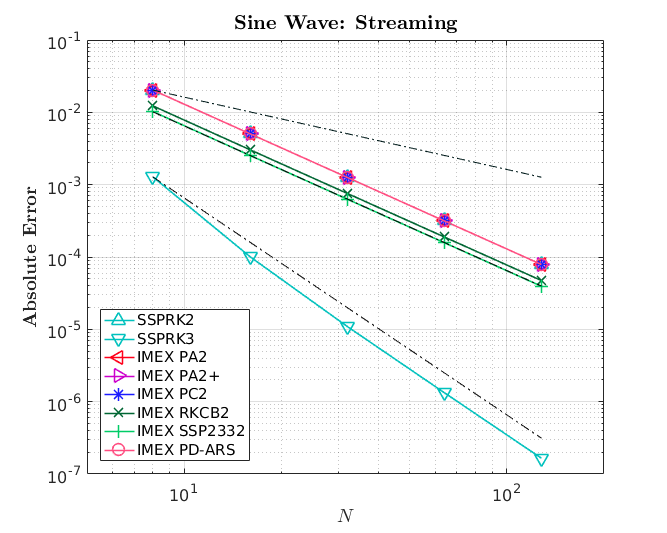
\includegraphics[width=\textwidth]{figures/SineWaveStreaming}
   \caption{Absolute error (cf. Eq.~\eqref{eq:errorNormAbsolute}) versus number of elements $N$ for the streaming sine wave test.  Results employing various time stepping schemes are compared: SSPRK2 (cyan triangles pointing up), SSPRK3 (cyan triangles pointing down), PA2 (red), PA2+ (purple), PC2 (blue), RKCB2 (dark green), SSP2332 (green), and PD-ARS (light red circles).  Black dash-dot reference lines are proportional to $N^{-1}$ (top), $N^{-2}$ (middle), and $N^{-3}$ (bottom), respectively.}
  \label{fig:SineWaveStreaming}
\end{figure}

\subsubsection{Sine Wave: Damping}

The next test we consider, adapted from \cite{skinnerOstriker_2013}, consists of a sine wave propagating with unit speed in a purely absorbing medium ($f_{0}=0$, $\sigma_{\Scatt}=0$), which results in exponential damping of the wave amplitude.  
We consider a periodic domain $D=\{x:x\in[0,1]\}$, and let the initial condition ($t=0$) be given as in Eq.~\eqref{eq:initialConditionStreaming}.  
For a constant absorption opacity $\sigma_{\Ab}$, the analytical solution at $t>0$ is given by
\begin{equation}
  \cJ(x,t)=\cJ_{0}(x-t)\times\exp(-\sigma_{\Ab} t)
  \quad\text{and}\quad
  \cH_{x}(x,t)=\cJ(x,t),
\end{equation}
where $\cJ_{0}(x)=\cJ(x,0)$.  

We compute numerical solutions for three values of the absorption opacity ($\sigma_{\Ab}=0.1$, $1$, and $10$), and adjust the end time $t_{\mbox{\tiny end}}$ so that $\sigma_{\Ab}t_{\mbox{\tiny end}}=10$, and the initial condition has been damped by factor $e^{-10}$.  
Thus, for $\sigma_{\Ab}=0.1$ the sine wave crosses the domain 100 times, while for $\sigma_{\Ab}=10$, it crosses the grid once.  

Figure~\ref{fig:SineWaveDamping} shows convergence results, obtained using different values of $\sigma_{\Ab}$, for various IMEX schemes at $t=t_{\mbox{\tiny end}}$.  
Results for $\sigma_{\Ab}=0.1$, $1$, and $10$ are plotted with red, green, and blue lines, respectively (see figure caption for further details).  
All the second-order accurate schemes (PA2, PA2+, RKCB2, and SSP2332) display second-order convergence rates (cf. bottom, black dash-dot reference line).  
For $\sigma_{\Ab}=0.1$, SSP2332 is the most accurate among these schemes, while PA2+ is the most accurate for $\sigma_{\Ab}=10$.  
On the other hand, PC2 and PD-ARS are indistinguishable and display at most first-order accurate convergence, as expected.  
(For $\sigma_{\Ab}=0.1$, PC2 and PD-ARS are the most accurate schemes for $N=8$ and $N=16$.)

\begin{figure}[H]
  \centering
    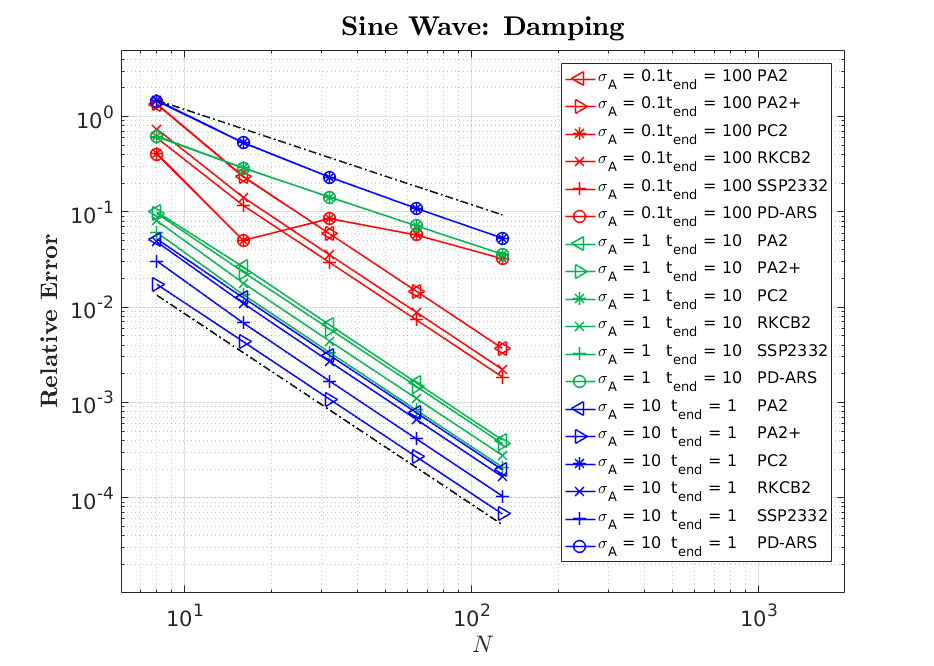
\includegraphics[width=\textwidth]{figures/SineWaveDamping}
   \caption{Relative error (cf. Eq.~\eqref{eq:errorNormRelative}) versus number of elements for the damping sine wave test.  Results for different values of the absorption opacity $\sigma_{\Ab}$, employing various IMEX time stepping schemes, are compared.  Errors for $\sigma_{\Ab}=0.1$, $1$, and $10$ are plotted with red, green, and blue lines, respectively.  The IMEX schemes employed are: PA2 (triangles pointing left), PA2+ (triangles pointing right), PC2 (asterisk), RKCB2 ($\times$), SSP2332 ($+$), and PD-ARS (circles).  Black dash-dot reference lines are proportional to $N^{-1}$ (top) and $N^{-2}$ (bottom), respectively.}
  \label{fig:SineWaveDamping}
\end{figure}

\subsubsection{Sine Wave: Diffusion}

The final test with known smooth solutions, adopted from \cite{radice_etal_2013}, is diffusion of a sine wave in a purely scattering medium ($f_{0}=0$, $\sigma_{\Ab}=0$).  
The computational domain $D=\{x:x\in[-3,3]\}$ is periodic, and the initial condition is given by
\begin{equation}
  \cJ_{0}(x)=0.5+0.49\times\sin\big(\f{\pi\,x}{3}\big)
  \quad\text{and}\quad
  \cH_{x,0}
  =-\f{1}{3\sigma_{\Scatt}}\pderiv{\cJ_{0}}{x}.  
  \label{eq:initialConditionDiffusion}
\end{equation}
For a sufficiently high scattering opacity, the moment equations limit to a diffusion equation for the number density (deviations appear at the $1/\sigma_{\Scatt}^{2}$-level).  
With the initial conditions in Eq.~\eqref{eq:initialConditionDiffusion}, the analytical solution to the limiting diffusion equation is given by
\begin{equation}
  \cJ(x,t)=\cJ_{0}(x)\times\exp\big(-\f{\pi^{2}\,t}{27\,\sigma_{\Scatt}}\big),
\end{equation}
and $\cH_{x}=(3\,\sigma_{\Scatt})^{-1}\pd{\cJ}{x}$.  
When computing errors for this test, we compare the numerical results obtained with the two-moment model to the analytical solution to the limiting diffusion equation.  
We compute numerical solutions using three values of the scattering opacity ($\sigma_{\Scatt}=10^{2}$, $10^{3}$, and $10^{4}$), and adjust the end time so that $t_{\mbox{\tiny end}}/\sigma_{\Scatt}=1$.  
The initial amplitude of the sine wave has then been reduced by a factor $e^{-\pi^{2}/27}\approx0.694$ for all values of $\sigma_{\Scatt}$.  

\begin{figure}[H]
  \centering
  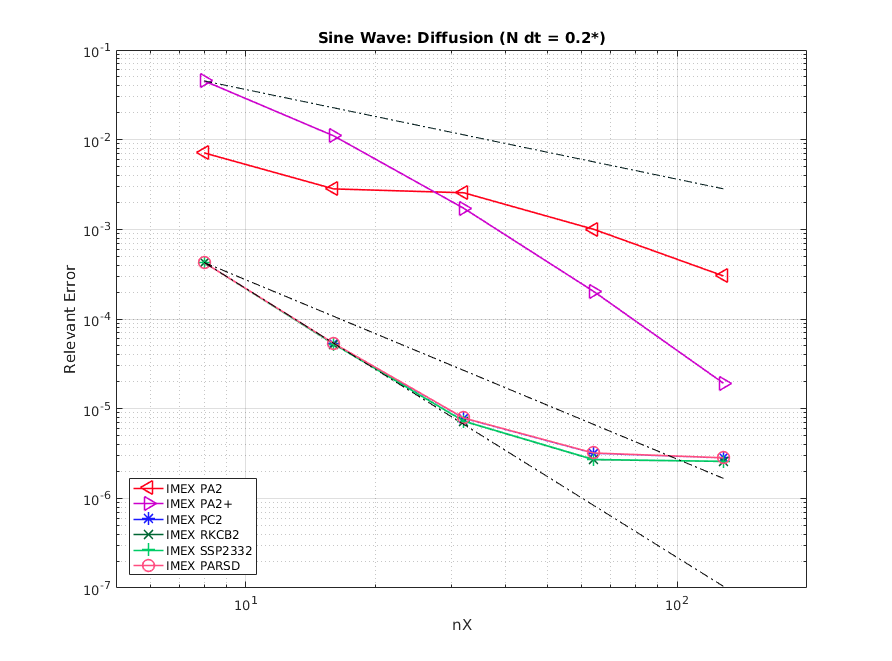
\includegraphics[width=1.0\textwidth]{figures/SineWaveDiffusionN}
   \caption{Absolute error (cf. Eq.~\eqref{eq:errorNormAbsolute}) for the number density $\cJ$ versus number of elements for the sine wave diffusion test.  Results with different values of the scattering opacity $\sigma_{\Scatt}$, employing different IMEX schemes, are compared.  Errors with $\sigma_{\Scatt}=10^{2}$, $10^{3}$, and $10^{4}$ are plotted with red, green, and blue lines, respectively.  The IMEX schemes employed are: PA2 (triangle pointing left), PA2+ (triangle pointing right), PC2 (asterisk), RKCB2 (cross), SSP2332 (plus), and PD-ARS (circle).  Black dash-dot reference lines are proportional to $N^{-1}$ (top) and $N^{-2}$ (bottom), respectively.}
  \label{fig:SineWaveDiffusionJ}
\end{figure}

\begin{figure}[H]
  \centering
  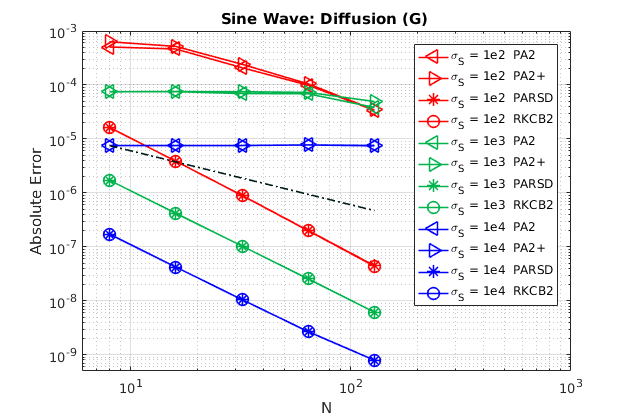
\includegraphics[width=1.0\textwidth]{figures/SineWaveDiffusionG}
   \caption{Same as in Figure~\ref{fig:SineWaveDiffusionJ}, but for the number flux $\cH_{x}$.}
  \label{fig:SineWaveDiffusionH}
\end{figure}

In Figures~\ref{fig:SineWaveDiffusionJ} and \ref{fig:SineWaveDiffusionH} we plot the absolute error, obtained using different values of $\sigma_{\Scatt}$, for various IMEX schemes at $t=t_{\mbox{\tiny end}}$.  
Results for $\sigma_{\Scatt}=10^{2}$, $10^{3}$, and $10^{4}$ are plotted with red, green, and blue lines, respectively (see figure caption for further details).  
(Scheme PC2 has been shown to work well for this test \cite{radice_etal_2013}, but is included here for comparison with the other IMEX schemes.)
Schemes PD-ARS, RKCB2, and SSP2332 are accurate for this test, and display third-order accuracy for the number density $\cJ$ and second-oder accuracy for $\cH_{x}$.  
For $\sigma=10^{2}$, the errors do not drop below $10^{-6}$ because of differences between the two-moment model and the diffusion equation used to obtain the analytic solution.  
For larger values of the scattering opacity, the two-moment model agrees better with the diffusion model, and we observe convergence over the entire range of $N$.  
Schemes PA2 and PA2+ do not perform well on this test (for reasons discussed in Section~\ref{sec:imex}).  
For $\sigma_{\Scatt}=10^{2}$, errors in $\cJ$ and $\cH_{x}$ decrease with increasing $N$, but for $\sigma_{\Scatt}=10^{4}$, errors remain constant with increasing $N$ over the entire range.  

\subsection{Packed Beam}
\label{sec:packedBeam}

Next we consider a one-dimensional test with discontinuous initial conditions.  
The purpose of this test is to further gauge the accuracy of the two-moment model and demonstrate the robustness of the DG scheme for dynamics close to the boundary of the realizable set $\cR$.  
The computational domain is $D=\{x:x\in[-1,1]\}$, and the initial condition is obtained from a distribution function given by
\begin{equation}
  f(x,\mu)
  =\left\{
  \begin{array}{cl}
    1        & \text{if} ~ x\le x_{\mbox{\tiny D}}, ~ \mu\ge\mu_{\mbox{\tiny D}} \\
    \delta & \text{if} ~ x\le x_{\mbox{\tiny D}}, ~ \mu<   \mu_{\mbox{\tiny D}} \\
    \delta & \text{otherwise},
  \end{array}
  \right.
\end{equation}
so that, with $\mu_{\mbox{\tiny D}}=0$, $\vect{\cM}\equiv\vect{\cM}_{\mbox{\tiny L}}=\big(0.5\,(1+\delta),0.25\,(1-\delta)\big)^{T}$ for $x\le x_{\mbox{\tiny D}}$, and $\vect{\cM}\equiv\vect{\cM}_{\mbox{\tiny R}}=\big(\delta,0\big)^{T}$ for $x> x_{\mbox{\tiny D}}$, where $\delta>0$ is a small parameter ($\delta\ll1$).  
We let $\delta=10^{-8}$, so that the initial conditions are very close to the boundary of the realizable domain (cf. Figure~\ref{fig:RealizableSetFermionic}).  
The analytical solution can be easily obtained by solving the transport equation for all angles $\mu$ (independent linear advection equations), and taking the angular moments.  
The numerical results shown in this section were obtained with the third-order scheme (polynomials of degree $k=2$ and the SSPRK3 time stepper) using $400$ elements.  
The time step is set to $\dt=0.1\times\dx$

Figure~\ref{fig:PackedBeam} shows results for various times obtained with the two-moment model.  
In the upper panels we plot the number density, while the number flux density is plotted in the lower panels.  
Numerical solutions are plotted with solid lines, while the analytical solution is plotted with dashed lines.  
In the left panels, the algebraic maximum entropy closure of Cernohorsky \& Bludman (CB) \cite{cernohorskyBludman_1994} (cf. Eqs.~\eqref{eq:eddingtonFactor} and \eqref{eq:closureMECB}) was used, while in the right panels the Minerbo closure (cf. Eqs.~\eqref{eq:eddingtonFactorLow} and \eqref{eq:closureMECB}) was used.  
For this test, the use of the realizability-preserving limiter described in Section~\ref{sec:limiter} was essential in order to avoid numerical problems.  
For the results obtained with the CB closure, the limiter was enacted whenever moments ventured outside the realizable set given by Eq.~\eqref{eq:realizableSet}.  
For the results obtained with the Minerbo closure, which is not based on Fermi-Dirac statistics, we used a modified limiter, which was enacted when the moments ventured outside the realizable domain of positive distributions; i.e., not bounded by $f < 1$, so that $\cJ > 0$ and $\cJ > \vect{\cH}|$ (e.g., \cite{levermore_1984}; see red line in Figure~\ref{fig:RealizableSetFermionic}).  

\begin{figure}[H]
  \centering
  \begin{tabular}{cc}
    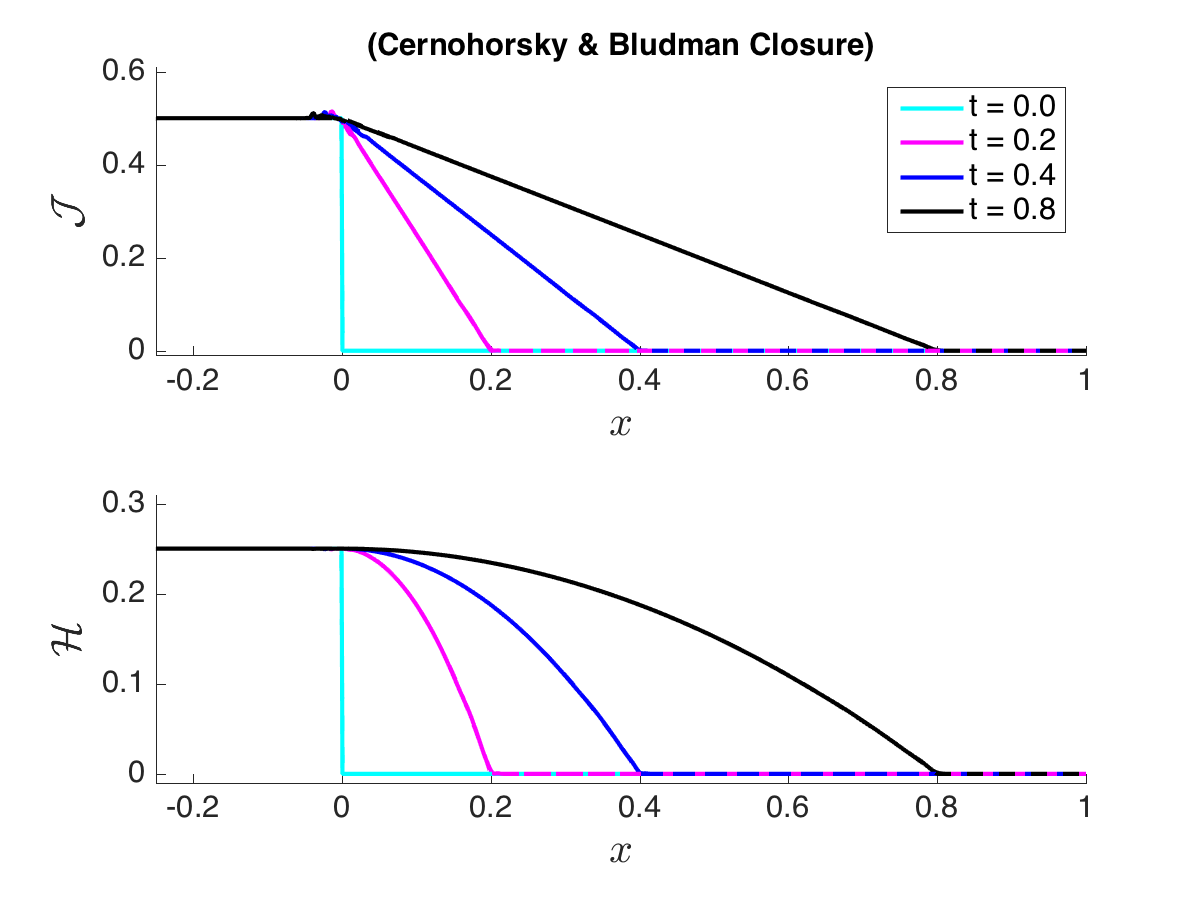
\includegraphics[width=0.5\textwidth]{figures/PackedBeam_ME_CB} &
    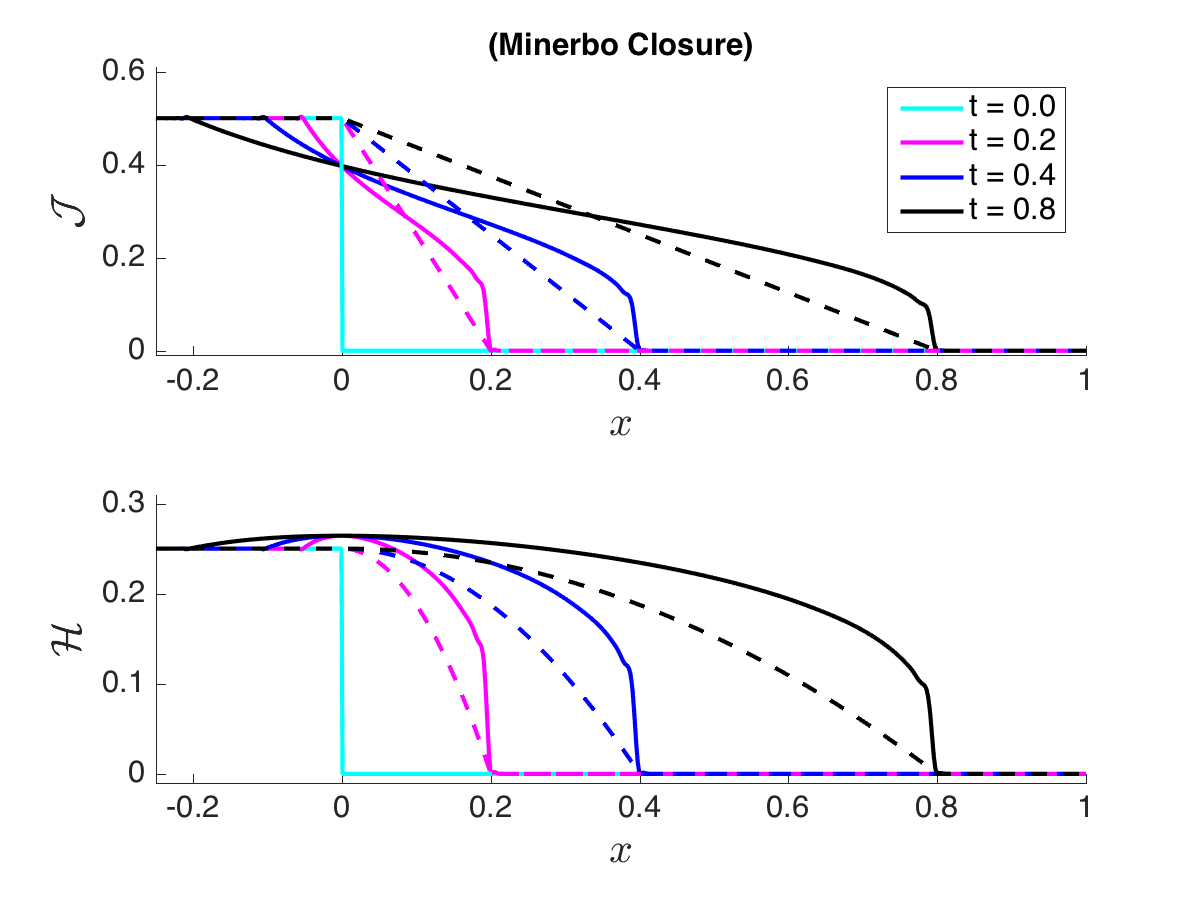
\includegraphics[width=0.5\textwidth]{figures/PackedBeam_ME_MI}
  \end{tabular}
   \caption{Numerical results from the packed beam problem at various times: $t=0$ (cyan), $t=0.2$ (magenta), $t=0.4$ (blue), and $t=0.8$ (black).  Results obtained with the Cernohorsky \& Bludman closure are displayed in the left panels, while results obtained with the Minerbo closure are displayed in the right panels.  The analytical solution (dashed lines) is also plotted.}
  \label{fig:PackedBeam}
\end{figure}

As can be seen in Figure~\ref{fig:PackedBeam}, with the CB closure the numerical solution obtained with the two-moment model tracks the analytic solution well, while with the Minerbo closure the numerical solution deviates substantially from the analytic solution.  
With the Minerbo closure, the solution also evolves outside the realizable domain for Fermi-Dirac statistics.  

In the left panel in Figure~\ref{fig:PackedBeam_Realizability} we plot $\gamma(\vect{\cM})=\big(1-\cJ\big)\,\cJ-|\vect{\cH}|$ versus position for various times.  
With the Minerbo closure, $\gamma(\vect{\cM})$ becomes negative in regions of the computational domain (dashed lines), while $\gamma(\vect{\cM})$ remains positive for all $x$ and $t$ the CB closure.  
In the right panel of Figure~\ref{fig:PackedBeam_Realizability} we plot the numerical solutions in the $(\cH,\cJ)$-plane.  
Initially, the moments are located in two points: $\vect{\cM}_{\mbox{\tiny L}}$ and $\vect{\cM}_{\mbox{\tiny R}}$, for $x\le0$ and $x>0$, respectively (marked by circles in Figure~\ref{fig:PackedBeam_Realizability}).  
For $t>0$, the solutions trace out curves in the $(\cH,\cJ)$-plane, connecting $\vect{\cM}_{\mbox{\tiny L}}$ and $\vect{\cM}_{\mbox{\tiny R}}$.  
With the CB closure, the solution curve (blue points) follows the boundary of the realizable set $\cR$ defined in Eq.~\eqref{eq:realizableSet} (cf. black line in Figure~\ref{fig:PackedBeam_Realizability}).  
With the Minerbo closure (magenta points), the solution follows a different curve --- outside the realizable domain for distribution functions bounded by $f\in(0,1)$, but inside the realizable domain of positive distributions (cf. red line in Figure~\ref{fig:PackedBeam_Realizability}).  
We have also run this test using the algebraic maximum entropy closure of Larecki \& Banach \cite{lareckiBanach_2011} and the simpler Kershaw-type closure in \cite{banachLarecki_2017a}.  
The numerical solutions obtained with both of these closures follow the analytic solution well, and remain within the realizable set $\cR$.  
We point out that simply using the realizability-preserving limiter described in Section~\ref{sec:limiter} with the Minerbo closure does not result in a realizability-preserving scheme for Fermi-Dirac statistics because of the properties of this closure discussed in Section~\ref{sec:algebraicClosure}, and plotted in the lower right panel of Figure~\ref{fig:MabWithDifferentClosure}.  

\begin{figure}[H]
  \centering
  \begin{tabular}{cc}
    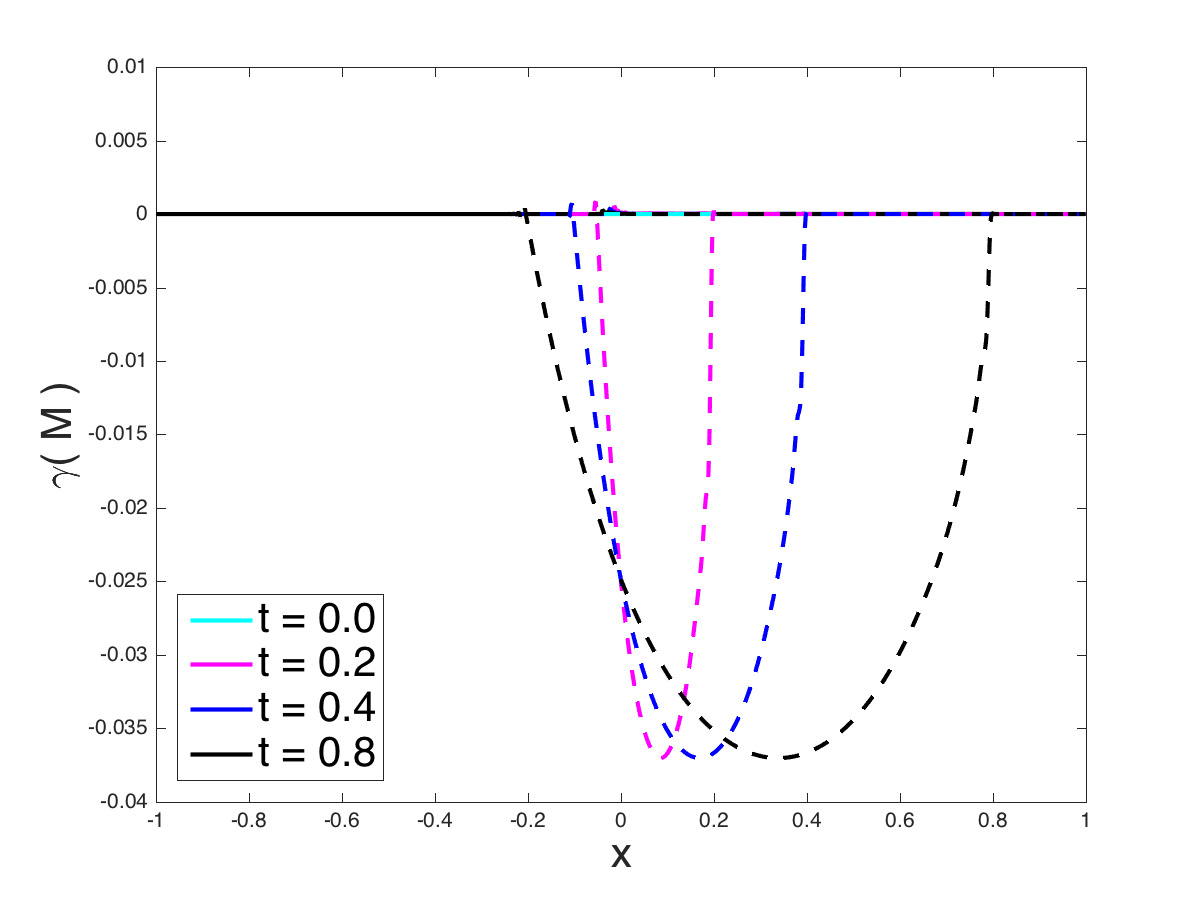
\includegraphics[width=0.485\textwidth]{figures/PackedBeam_Realizability} &
    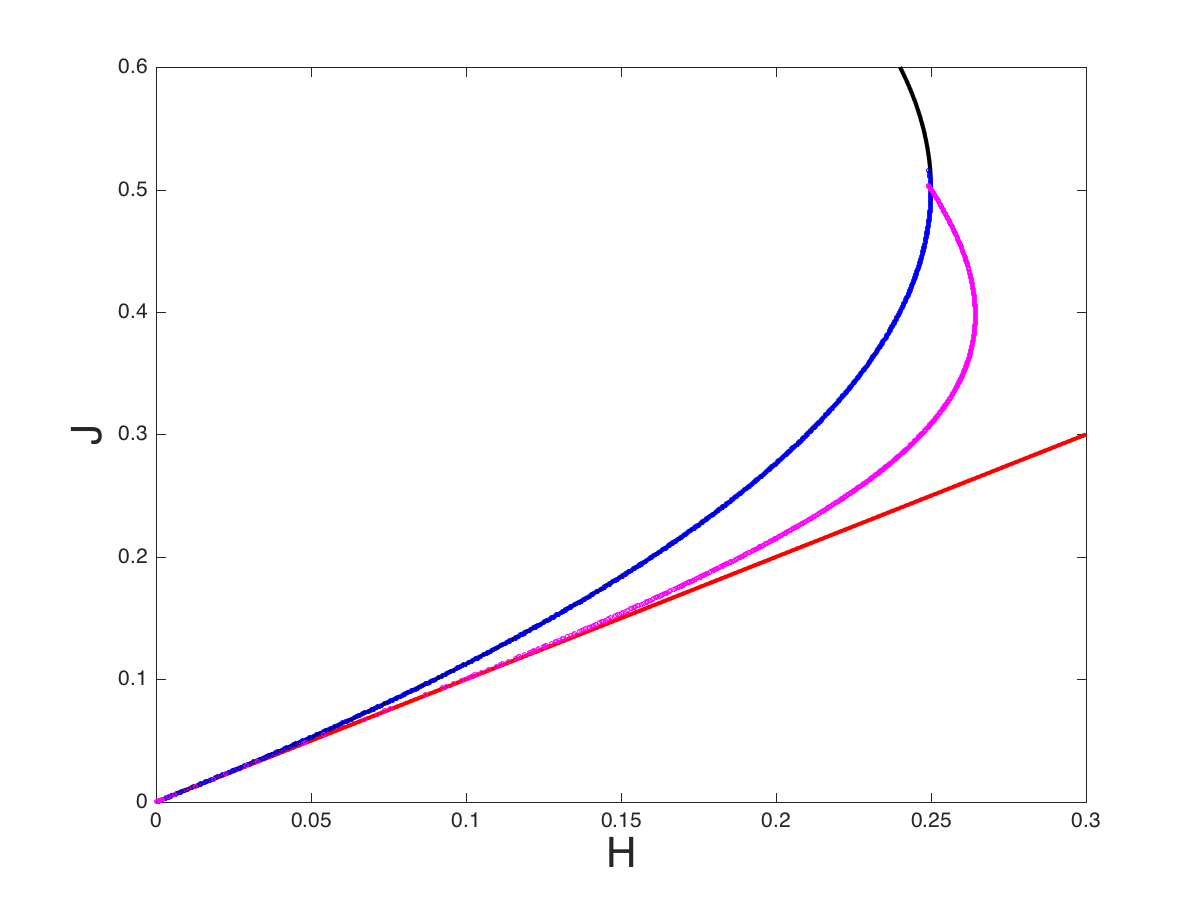
\includegraphics[width=0.485\textwidth]{figures/PackedBeam_RealizableDomain}
  \end{tabular}
   \caption{In the left panel, $\gamma(\vect{\cM})=(1-\cJ)\,\cJ-|\vect{\cH}|$ is plotted versus $x$ for various times in the packed beam problem: $t=0$ (cyan), $t=0.2$ (magenta), $t=0.4$ (blue), and $t=0.8$ (black).  Results obtained with the CB closure, which remain positive throughout the evolution, are plotted with solid lines, while results obtained with the Minerbo closure are plotted with dashed lines.  In the right panel, the moments are plotted in the $(\cH,\cJ)$-plane for the same times as in the left panel.  Results obtained with the CB and Minerbo closures are plotted in blue and magenta, respectively.  The solid black and red lines are contours where $(1-\cJ)\,\cJ=\cH$ and $\cJ=\cH$, respectively.  The initial states are marked with black circles.}
  \label{fig:PackedBeam_Realizability}
\end{figure}

\subsection{Fermion Implosion}
\label{sec:fermionImplosion}

The next test is inspired by line source benchmark (cf. \cite{brunner_2002,garrettHauck_2013}), which is a challenging test for approximate transport algorithms.  
The original line source test consists of an initial delta function particle distribution in radius $R=|\vect{x}|$; i.e., $f_{0}=\delta(R)$.  
For $t>0$, a radiation front propagates in the radial direction, away from $R=0$.  
Apart from capturing details of the exact transport solution, maintaining realizability of the two-moment solution is challenging.  

Here, a modified version of the line source --- dubbed \emph{Fermion Implosion},  designed to test the realizability-preserving properties of the two-moment model for fermion transport --- is computed on a two-dimensional domain $D=\{\vect{x}\in\bbR^{2}:x^{1}\in[-1.28,1.28], x^{2}\in[-1.28,1.28]\}$.  
Instead of initializing with a delta function, we follow the initialization procedure in \cite{garrettHauck_2013}, and approximate the initial condition using an isotropic Gaussian distribution function.  
However, different from \cite{garrettHauck_2013}, the initial distribution function is bounded $f_{0}\in(0,1)$, and reaches a minimum in the center of the computational domain (hence implosion)
\begin{equation}
  f_{0}
  =1-\max\Big[\,e^{-R^{2}/(2\,\sigma_{0}^{2})},10^{-8}\,\Big].  
\end{equation}
We set $\sigma_{0}=0.03$, and evolve to a final time of $t=1.0$.  
We run this test using a grid of $512^{2}$ elements, polynomials of degree $k=1$, and the SSPRK2 time stepping scheme with $\dt=0.1\times\dx^{1}$.  
(There are no collisions included in this test; i.e., $\sigma_{\Ab}=\sigma_{\Scatt}=0$.)  
For comparison, we present results using the algebraic closures of Cernohorsky \& Bludman (CB) and Minerbo.  

\begin{figure}[H]
  \centering
  \begin{tabular}{cc}
    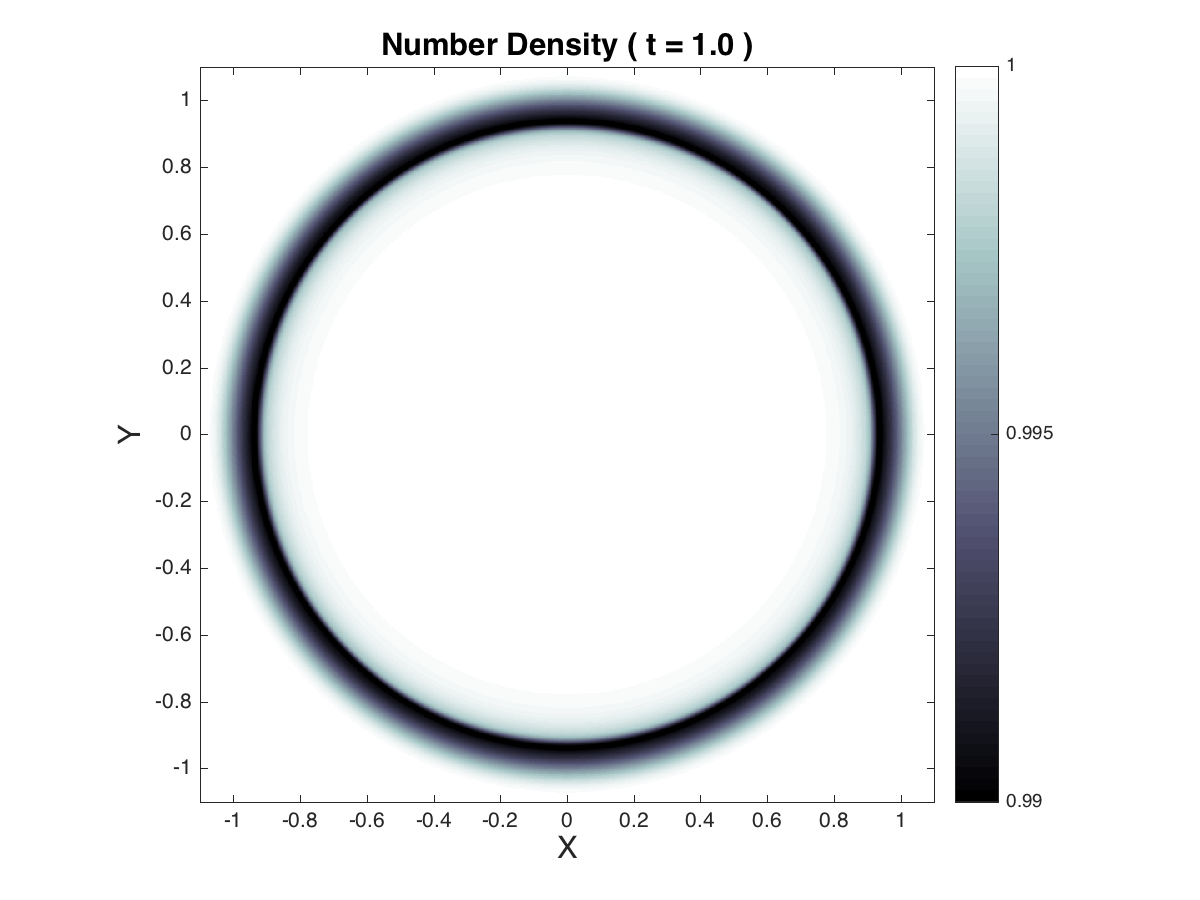
\includegraphics[width=0.495\textwidth]{figures/Implosion_Image} &
    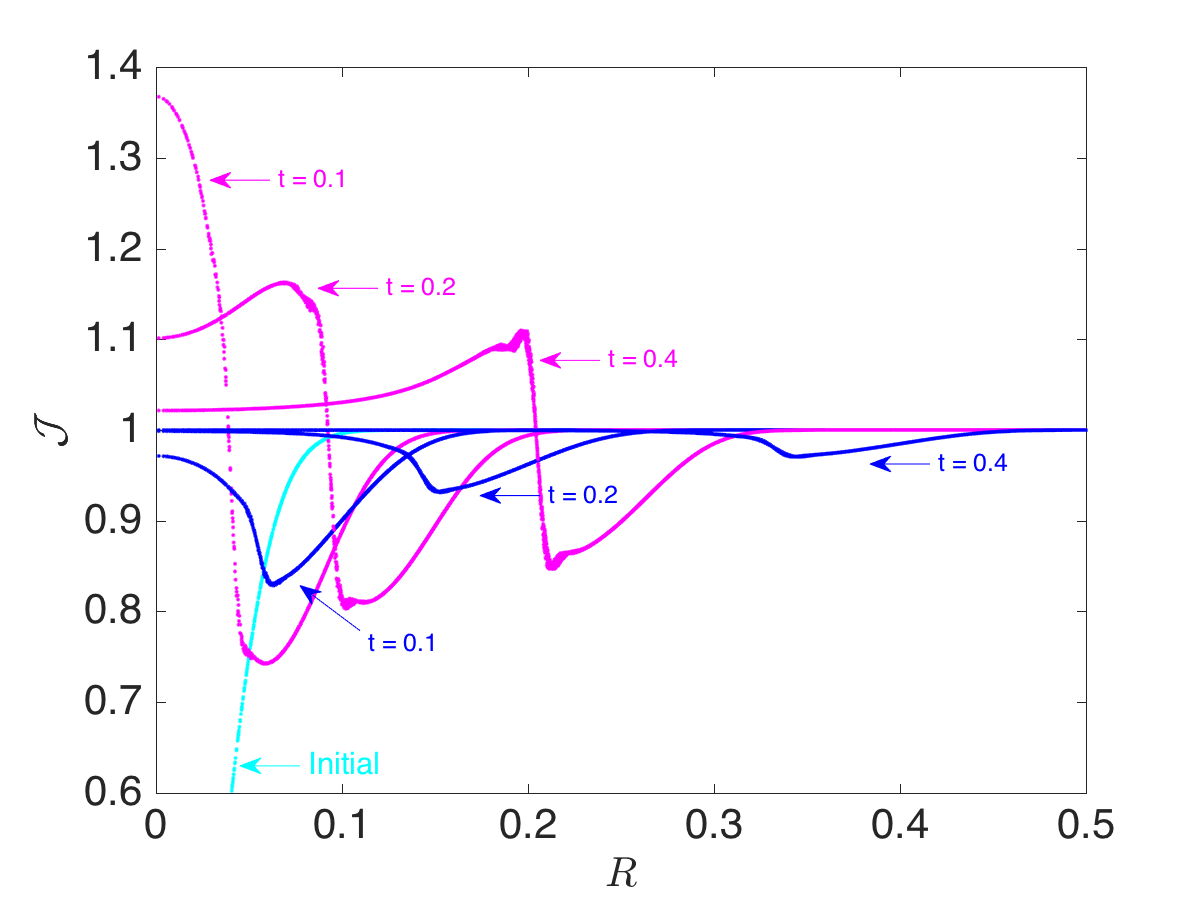
\includegraphics[width=0.495\textwidth]{figures/Implosion_Lineout} \\
    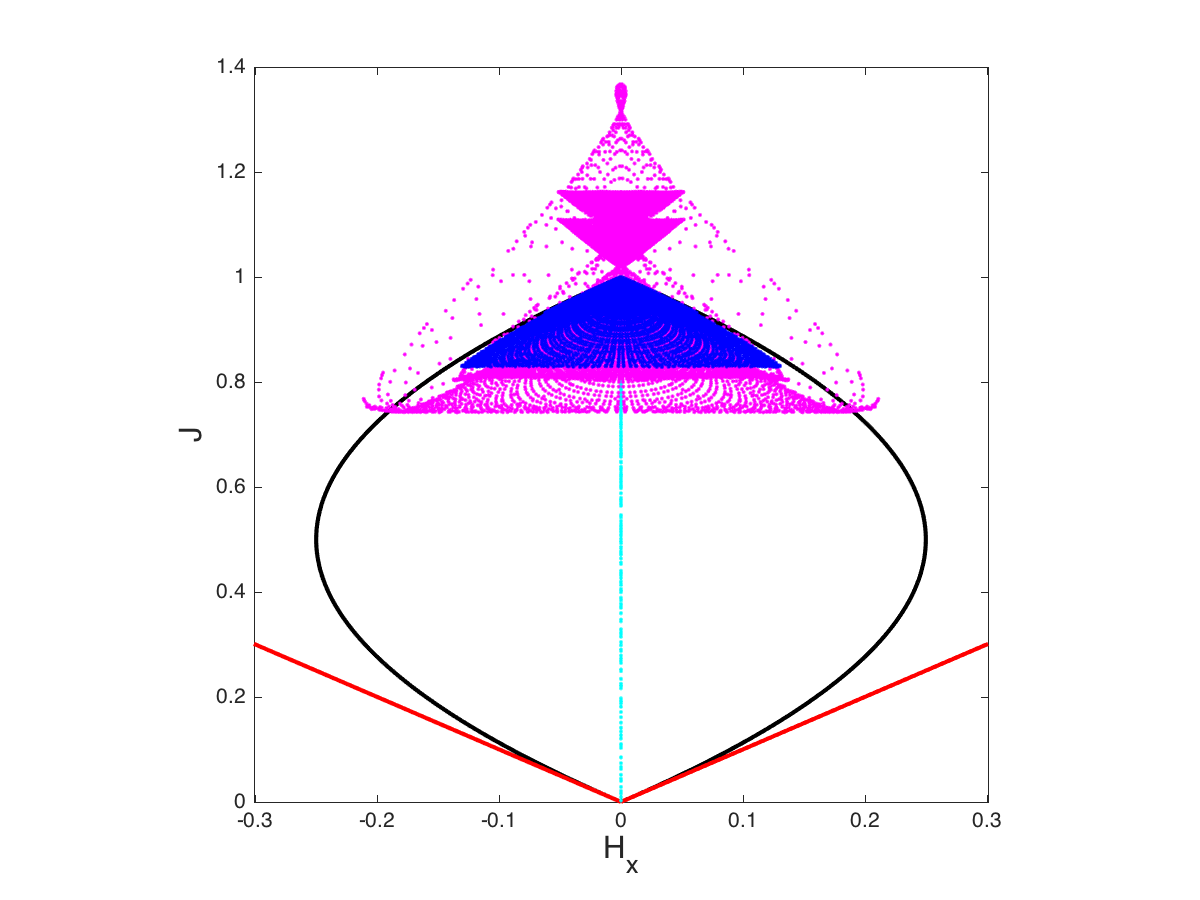
\includegraphics[width=0.495\textwidth]{figures/Implosion_RealizableDomain} &
    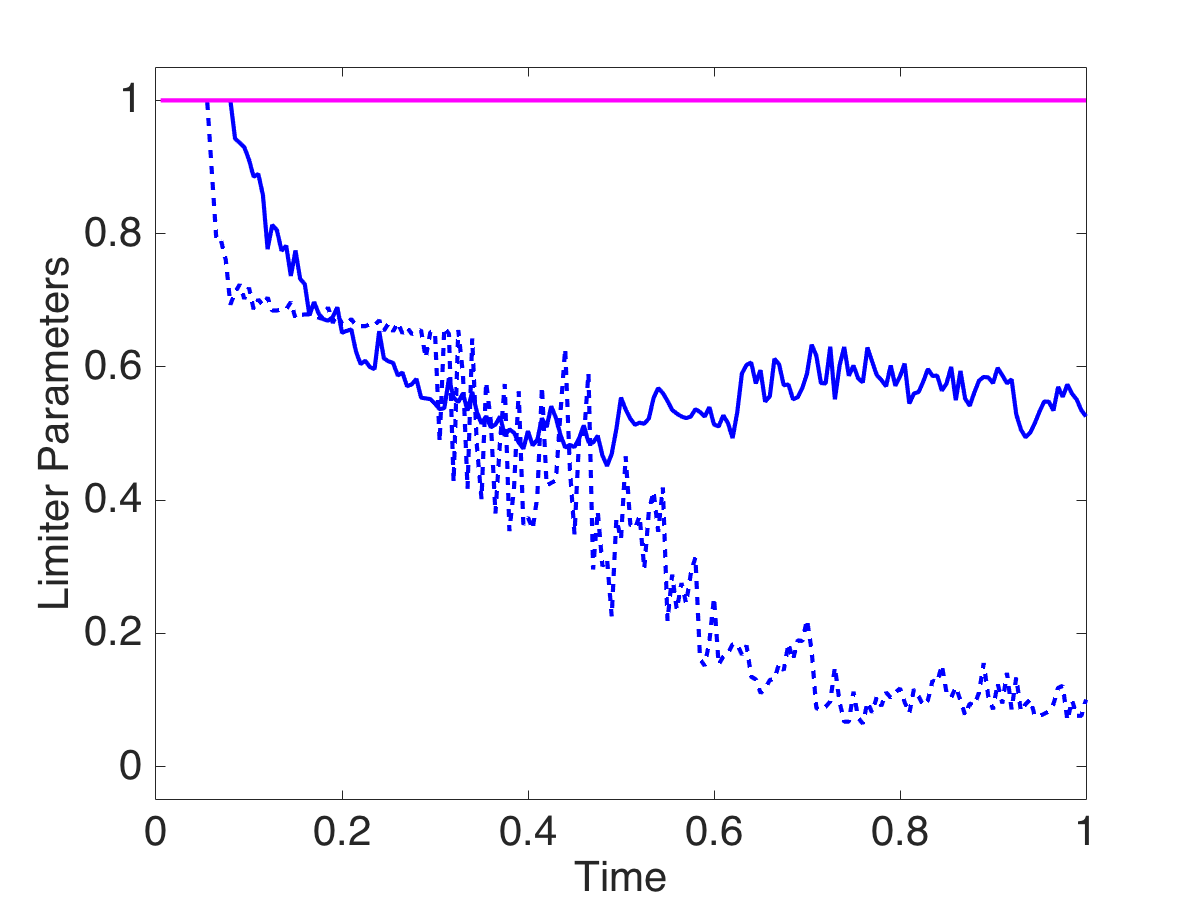
\includegraphics[width=0.495\textwidth]{figures/Implosion_LimiterParameters}
  \end{tabular}
   \caption{Numerical results for the Fermion Implosion problem, computed both the CB and Minerbo closures.  Spatial distribution of the number density $\cJ$ (CB closure only) at $t=1$ (upper left panel).  In the upper right panel we plot the number density $\cJ$ versus radius $R=|\vect{x}|$ for various times ($t=0$, $0.1$, $0.2$, and $0.4$) for the CB (blue), the Minerbo (magenta) closures, and the reference transport solution (dashed black lines).  (The initial condition, which is the same for all models, is plotted with cyan.)  Numerical solutions in the $(\cH_{x},\cJ)$-plane (lower left panel), for the same times as plotted in the upper right panel are plotted for CB and Minerbo.  Limiter parameters $\vartheta_{1}$ (solid) and $\vartheta_{2}$ (dashed) in Section~\ref{sec:limiter} (minimum over the whole computational domain) versus time (lower right panel).}
  \label{fig:Implosion}
\end{figure}

Numerical results for the Fermion Implosion problem are plotted in Figure~\ref{fig:Implosion}.  
For $t>0$, the low-density region in the center of the computational domain is quickly filled in, and a cylindrical perturbation propagates radially away from the center.  
For the model with the CB closure, this perturbation, seen as a depression in the density relative to the ambient medium, has reached $R\approx1$ for $t=1$ (upper left panel in Figure~\ref{fig:Implosion}).  
The right panel in Figure~\ref{fig:Implosion} illustrates the difference in dynamics resulting from the two closures.  
(We also plot a reference transport solution obtained using the filtered spherical harmonics scheme described in \cite{garrettHauck_2013}; dashed black lines.\footnote{Kindly provided by Dr. Ming Tse Paul Laiu (private communications).})  
With the CB closure (blue lines), the central density increases towards the maximum value of unity, and an low-density pulse propagates radially.  
The amplitude of the pulse decreases with time due to the geometry of the problem.  
For $t=0.4$, the peak depression in located around $R=0.34$ (with $\cJ\approx0.96$).  
With the Minerbo closure, the central density continues to increase beyond unity, and reaches a maximum of about $\cJ\approx1.37$ at $t=0.1$.  
The central density starts to decrease beyond this point in time, and a steepening pulse propagates radially away from the center.  
(This pulse is trailing the pulse in the model computed with the CB closure.)  
At $t=0.4$, a discontinuity appears to have formed around $R=0.2$, resulting in numerical oscillations.  
Except for the realizability-enforcing limiter (which is not triggered for this model), no other limiters are used to prevent numerical oscillations.  
Although the solutions obtained with the two-moment model differ from the reference transport solution, the results obtained with the CB closure are in closer agreement with the transport solution.  
This is likely because the CB closure is consistent with the bound $f<1$ satisfied by the transport solution in this test.  
(For tests involving lower occupancies, the CB and Minerbo closures are expected to perform similarly.)  
In the lower left panel in Figure~\ref{fig:Implosion}, the moments are plotted in the $(\cH_{x},\cJ)$-plane for the same times as plotted in the upper left panel.  
(Each dot represents the moments at a specific spatial point and time.)  
Initially, $\vect{\cH}=0$, and all the moments lie on the line connecting $(0,0)$ and $(0,1)$; cyan points.  
With the CB closure (blue points), the moments are confined to evolve inside the realizable domain $\cR$ (black), while with the Minerbo closure, the moments are not confined to $\cR$, but to the region above the red lines (the realizable domain for moments of positive distribution functions), and this is the reason for the difference in dynamics in the two models.  
For the model with the CB closure, some moments evolve very close to the boundary of the realizable domain, and the positivity limiter is continuously triggered to damp these moments towards the cell average, which is realizable by the design of the numerical scheme.  
In the lower right panel in Figure~\ref{fig:Implosion} we plot the limiter parameters $\vartheta_{1}$ (solid) and $\vartheta_{2}$ (dashed) (cf. \eqref{eq:limitDensity} and \eqref{eq:limitMoments}) versus time for the CB closure model (blue) and the Minerbo closure model (magenta); the minimum over the whole computational domain is plotted.  
For the CB closure model, the limiter is triggered to prevent both density overshoots and $\gamma(\cM)<0$.  
Late in the simulation ($t\gtrsim0.7$), the minimum value of $\vartheta_{2}$ is around $0.1$.  
For the model using the Minerbo closure, the limiter is not triggered ($\vartheta_{1}=\vartheta_{2}=1$).  

\subsection{Homogeneous Sphere}
\label{sec:homogeneousSphere}

The homogeneous sphere test (e.g., \cite{smit_etal_1997}) considers a sphere with radius $R$.  
Inside the sphere (radius $<R$), the absorption opacity $\sigma_{\Ab}$ and the equilibrium distribution function $f_{0}$ are set to constant values.  
The scattering opacity $\sigma_{\Scatt}$ is set to zero in this test (i.e., $\xi=1$).  
Outside the sphere, the absorption opacity is zero.  
The steady state solution, obtained by solving the transport equation in spherical symmetry, is given by
\begin{equation}
  f_{\mbox{\tiny A}}(r,\mu)=f_{0}\,\big(1-e^{-\chi_{0}\,s(r,\mu)}\big),
  \label{eq:distributionHomogeneousSphere}
\end{equation}
where $r=|\vect{x}|$, 
\begin{equation}
  s(r,\mu)
  =\left\{
  \begin{array}{lll}
    r\,\mu+R\,g(r,\mu) & \mbox{if}\quad r<R, & \mu\in[-1,+1], \\
    2\,R\,g(r,\mu) & \mbox{if}\quad r \ge R, & \mu\in[(1-(R/r)^{2})^{1/2},+1], \\
    0 & \mbox{otherwise},
  \end{array}
  \right.
\end{equation}
and $g(r,\mu)=[1-(r/R)^{2}(1-\mu^{2})]^{1/2}$.  
Thus, $f_{\mbox{\tiny A}}(r,\mu)\in(0,f_{0})~\forall~r,\mu$.  

Here, this test is computed using a three-dimensional Cartesian domain $D=\{\vect{x}\in\bbR^{3}:x^{1}\in[0,2], x^{2}\in[0,2], x^{3}\in[0,2]\}$.  
Because of the symmetry of the problem, and to save computational resources, we only compute the solution in one octant.  
On the inner boundaries, we impose reflecting boundary conditions, while we impose 'homogeneous' boundary conditions on the outer boundary in all three coordinate dimensions; i.e., values for all moments in a boundary element are set equal to the corresponding values in the nearest element just inside $D$.  
Since this test is computed with Cartesian coordinates using a relatively low spatial resolution ($64^{3}$), we have found it necessary to smooth out the opacity over a finite radial extent to avoid numerical artifacts due to a discontinuous absorption opacity.  
Specifically, we use an absorption opacity of the following form
\begin{equation}
  \sigma_{\Ab}(r)=\f{\sigma_{\Ab,0}}{(r/R_{0})^{p}+1}.  
\end{equation}
We set $f_{0}=1$, and compute three versions of this test: one with $\sigma_{\Ab,0}=1$, $R_{0}=1$, and $p=80$ (Test~A), one with $\sigma_{\Ab,0}=10$, $R_{0}=1$, and $p=80$ (Test~B), and one with $\sigma_{\Ab}=10^{3}$, $R_{0}=0.85$, and $p=40$ (Test~C).  
(These values for $R_{0}$ and $p$ result in similar radius for where the optical depth equals $2/3$ in Test~B and Test~C.)
We compute until $t=5$, when the system has reached an approximate steady state.  
In all the tests, we use the IMEX scheme PD-ARS with $\dt=0.1\times\dx^{1}$ --- the least compute-intensive of the convex-invariant IMEX schemes presented here.  
The main purpose of this test is to compare the results obtained using the different algebraic closures discussed in Section~\ref{sec:algebraicClosure}.  

In Figure~\ref{fig:HomogeneousSphere}, we plot results obtained for all tests at $t=5$: Test~A (top panels), Test~B (middle panels), and Test~C (bottom panels).  
The particle density $\cJ$ and the flux factor $h=|\vect{\cH}|/\cJ$ (left and right panels, respectively) are plotted versus radius $r=|\vect{x}|$.  
In each panel, results obtained with the various algebraic closures discussed in Section~\ref{sec:algebraicClosure} are plotted: Minerbo (magenta), CB (blue), BL (green), and Kershaw (cyan).  
The analytical solution is also plotted (dashed black lines).  
\begin{figure}[H]
  \centering
  \begin{tabular}{cc}
    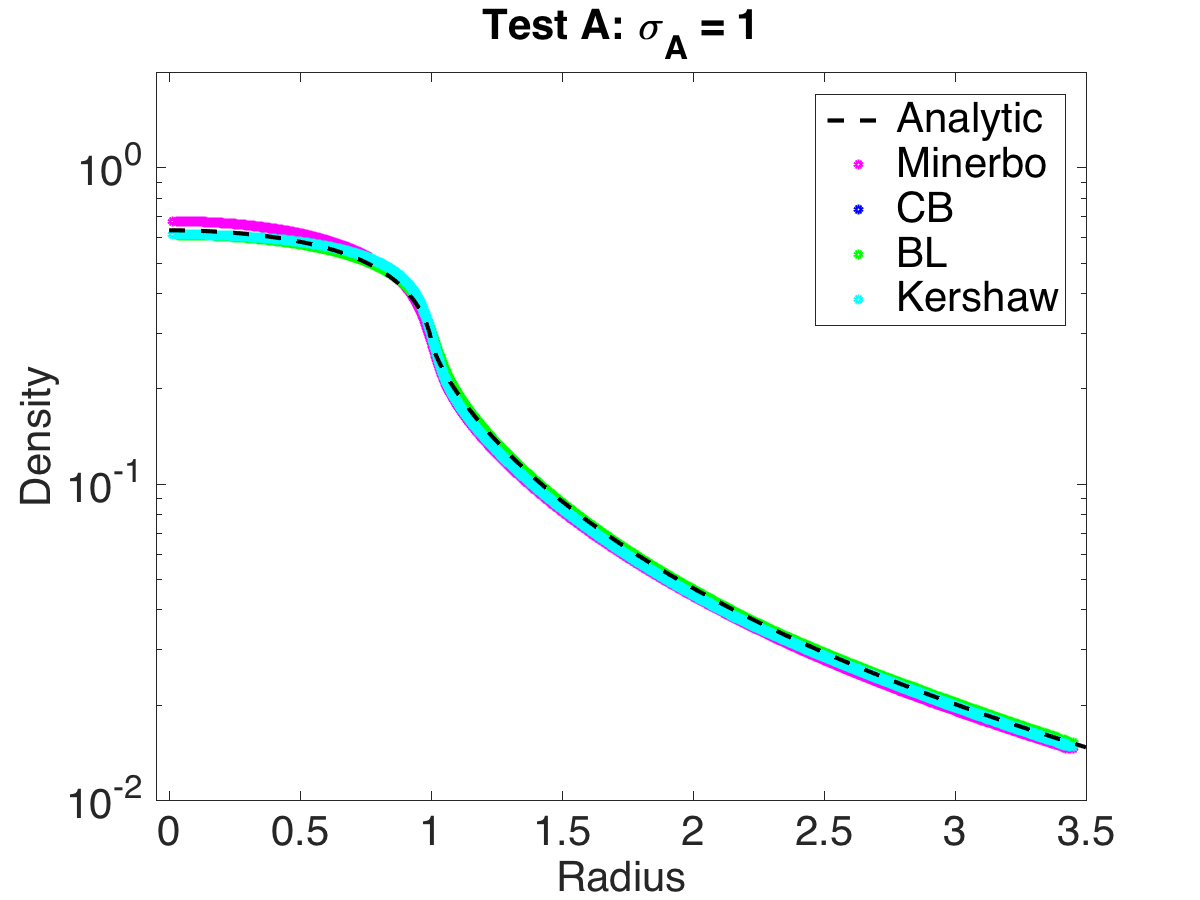
\includegraphics[width=0.5\textwidth]{figures/HomogeneousSphere_ClosureComparison_Chi_1e0_Density}
    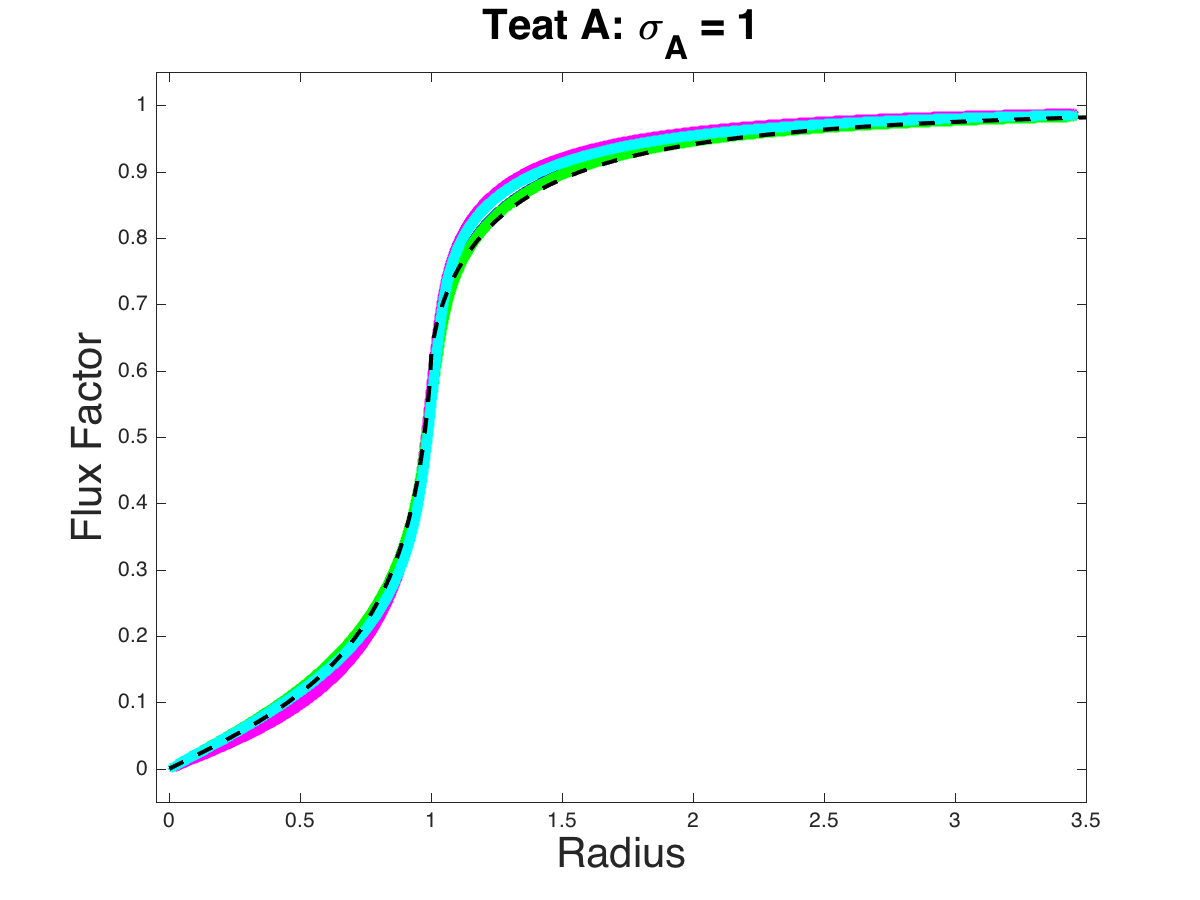
\includegraphics[width=0.5\textwidth]{figures/HomogeneousSphere_ClosureComparison_Chi_1e0_FluxFactor} \\
    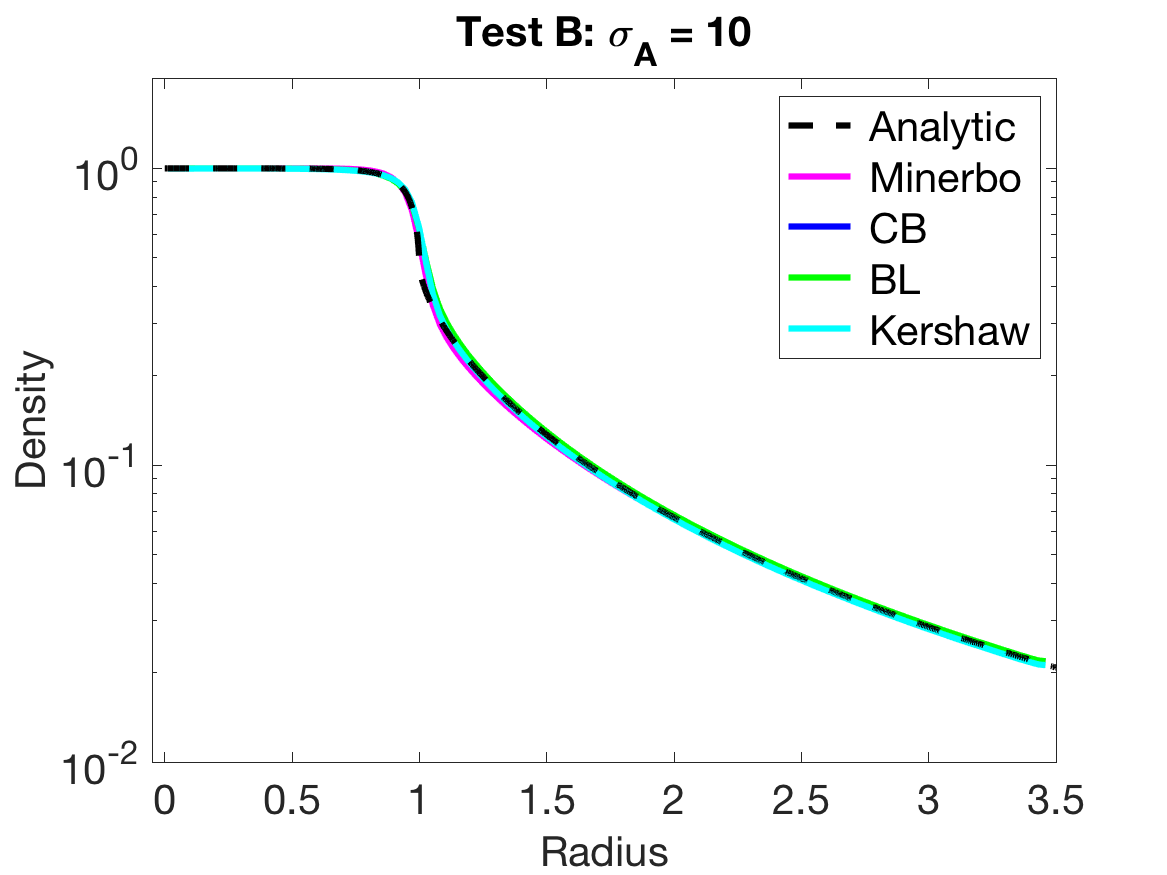
\includegraphics[width=0.5\textwidth]{figures/HomogeneousSphere_ClosureComparison_Chi_1e1_Density}
    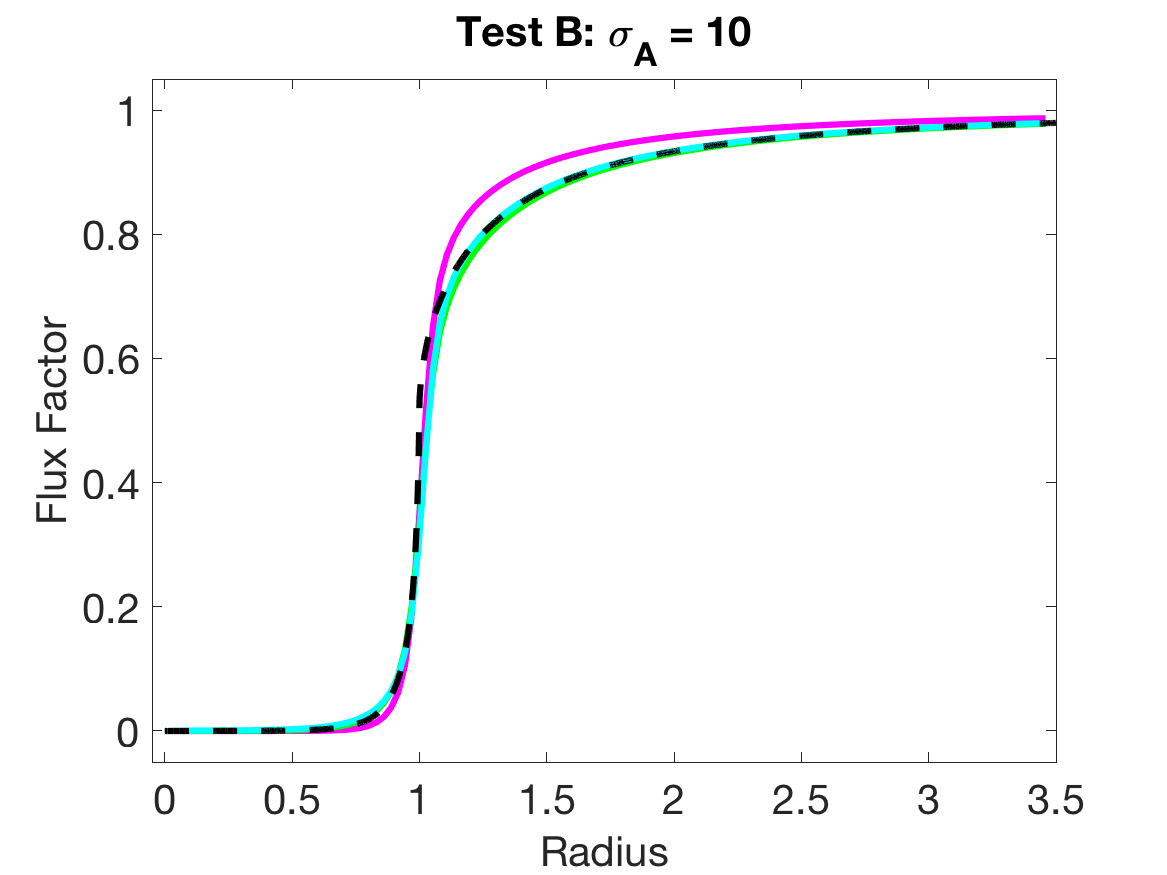
\includegraphics[width=0.5\textwidth]{figures/HomogeneousSphere_ClosureComparison_Chi_1e1_FluxFactor} \\
    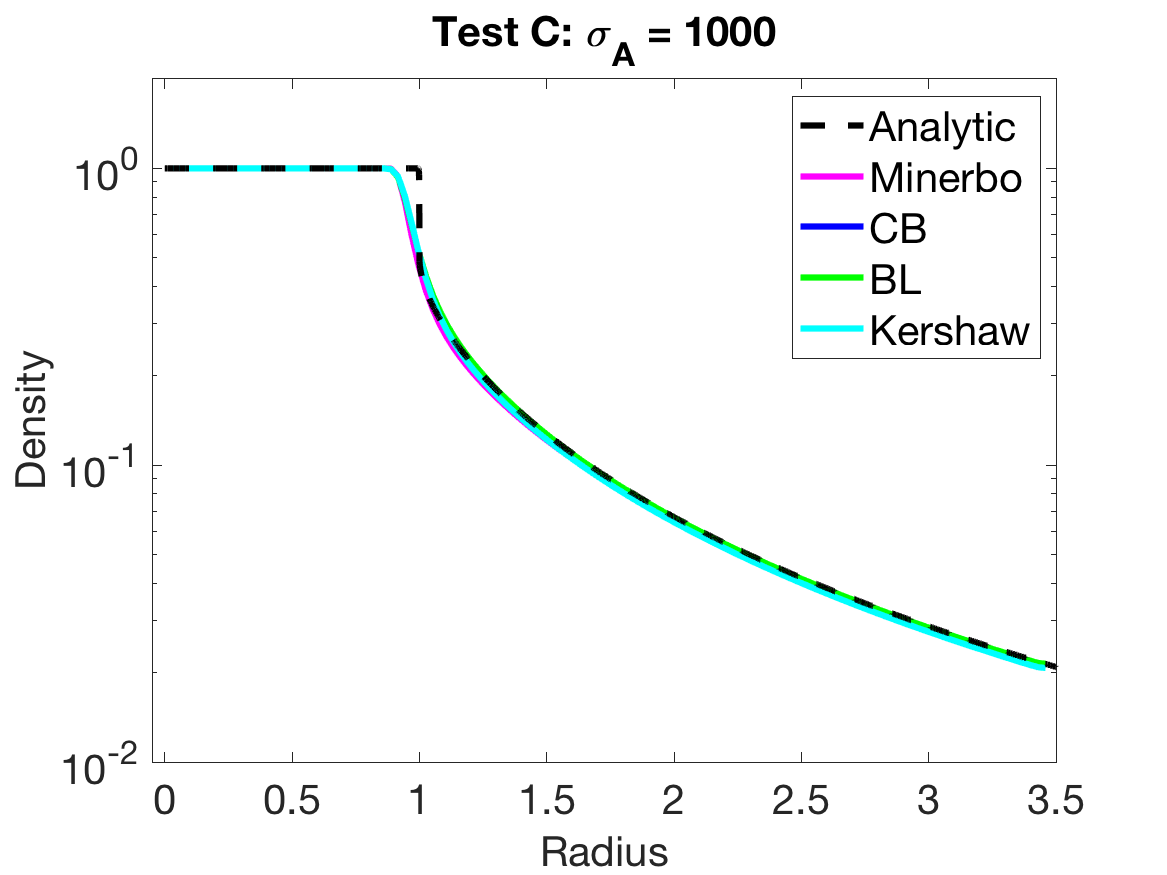
\includegraphics[width=0.5\textwidth]{figures/HomogeneousSphere_ClosureComparison_Chi_1e3_Density}
    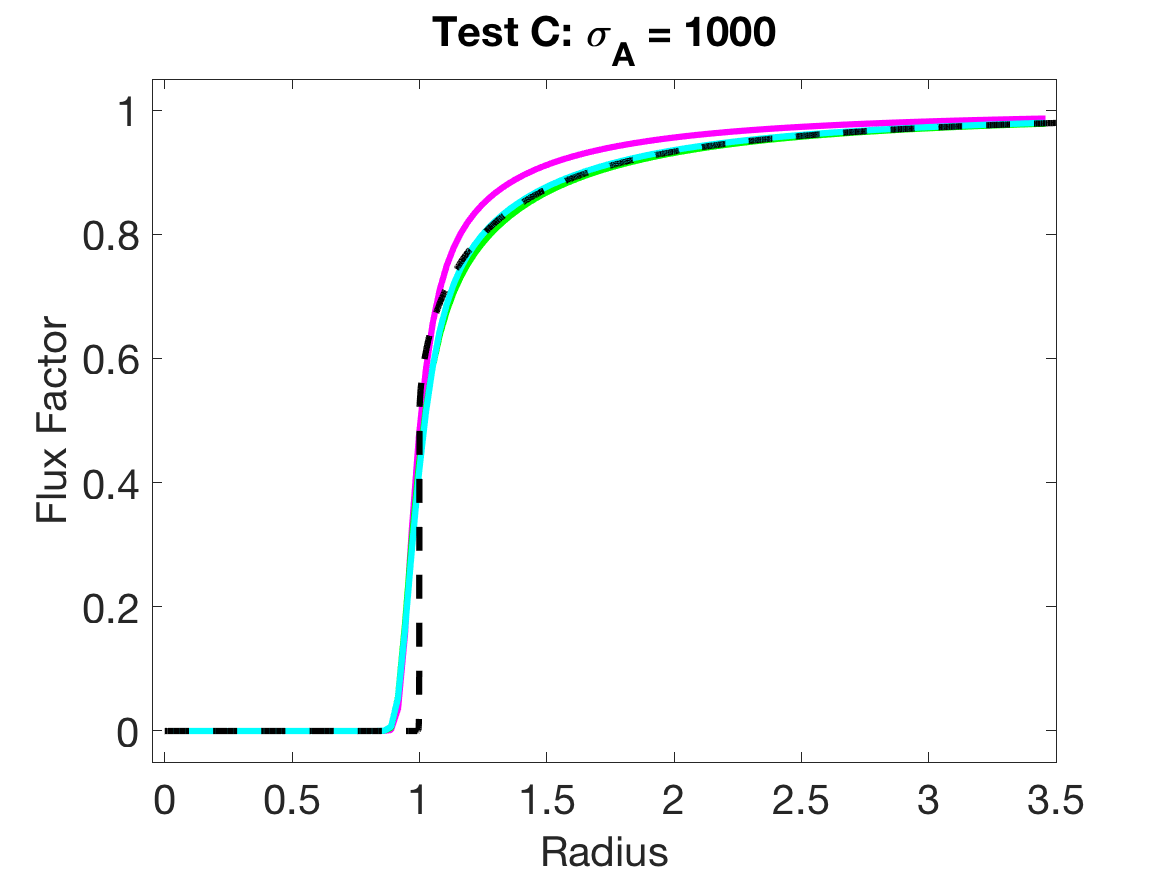
\includegraphics[width=0.5\textwidth]{figures/HomogeneousSphere_ClosureComparison_Chi_1e3_FluxFactor}
  \end{tabular}
   \caption{Results obtained for the homogeneous sphere problem with the two-moment model for different values of the absorption opacity $\sigma_{\Ab,0}$: $1$ (top panels), $10$ (middle panels), and $1000$ (bottom panels).  The particle density (left panels) and the flux factor (right panels) are plotted versus radius.  Numerical results obtained with the algebraic closures of Minerbo (magenta), CB (blue), BL (green), and Kershaw (cyan) are compared with the analytic solution (dashed black lines).}
  \label{fig:HomogeneousSphere}
\end{figure}

We find good overall agreement between the results obtained with the two-moment model and the analytical solution.  
Partly due to the smoothing of the absorption opacity around the surface, the numerical and analytical solutions naturally differ around $r=1$.  
Aside from some differences discussed in more detail below, the numerical and analytical solutions --- for all values of the absorption opacity $\sigma_{\Ab,0}$ and all closures --- agree well as $r$ tends to zero, as well as when $r\gg1$.  
The results obtained with the maximum entropy closures CB and BL are practically indistinguishable on the plots.  
This is consistent with the similarity of the Eddington factors for these two closures, as shown in Figure~\ref{fig:EddingtonFactorsWithDifferentClosure}.  
We also find that the results obtained with the fermionic Kershaw closure agree well with the maximum entropy closures based on Fermi-Dirac statistics (CB and BL).  
From the plots of the particle density (left panels in Figure~\ref{fig:HomogeneousSphere}), the results obtained with all the closures, including Minerbo, appear very similar.  
(For Test~A, the particle density obtained with the Minerbo closure deviates the most from the analytic solution inside $r\approx0.75$; upper left panel).  
From the plots of the flux factor (right panels in Figure~\ref{fig:HomogeneousSphere}), it is evident that the results obtained with the Minerbo closure --- the only closure not based on Fermo-Dirac statistics --- deviates the most from the analytic solution outside $r=1$, where the flux factor is consistently higher than the analytical solution for all values of $\sigma_{\Ab,0}$.  
The fermionic closures (CB, BL, and Kershaw) track the analytic solution better.  
Similar agreement between the numerical and analytical solutions was reported by Smit et al. \cite{smit_etal_1997}, when using the CB maximum entropy closure with $f_{0}=0.8$ and an unsmoothed absorption opacity $\sigma_{\Ab}=4$.  
We also note that our results appear to be somewhat at odds with the results recently reported by Murchikova et al. \cite{murchikova_etal_2017}, who compared results obtained with the two-moment model using a large number of algebraic closures for this same problem (albeit using an unsmoothed and slightly different value for the absorption opacity).  
Murchikova et al. do not plot the particle density, but find essentially no difference in the flux factor and the Eddington factor when comparing results obtained with the maximum entropy closures of Minerbo and Cernohorsky \& Bludman (CB).  

In Figure~\ref{fig:HomogeneousSphereRealizability}, we further compare the results obtained when using the Minerbo and CB closures by plotting the solutions to the homogeneous sphere problem for Test~C at $t=5$ in the $(\cH_{1},\cJ)$-plane (cf. the realizable domain in Figure~\ref{fig:RealizableSetFermionic}).  
The numerical solution at each spatial point is represented by a magenta dot in the panels.  
Results obtained using the CB closure are plotted in the upper left panel, while results obtained using the Minerbo closure are plotted in the upper right panel.  
In the lower two panel we zoom in on the results obtained with the Minerbo closure around the top and lower right regions of the realizable domain (lower left and lower right panel, respectively; cf. blue boxes in the upper right panel).  
\begin{figure}[H]
  \centering
  \begin{tabular}{cc}
    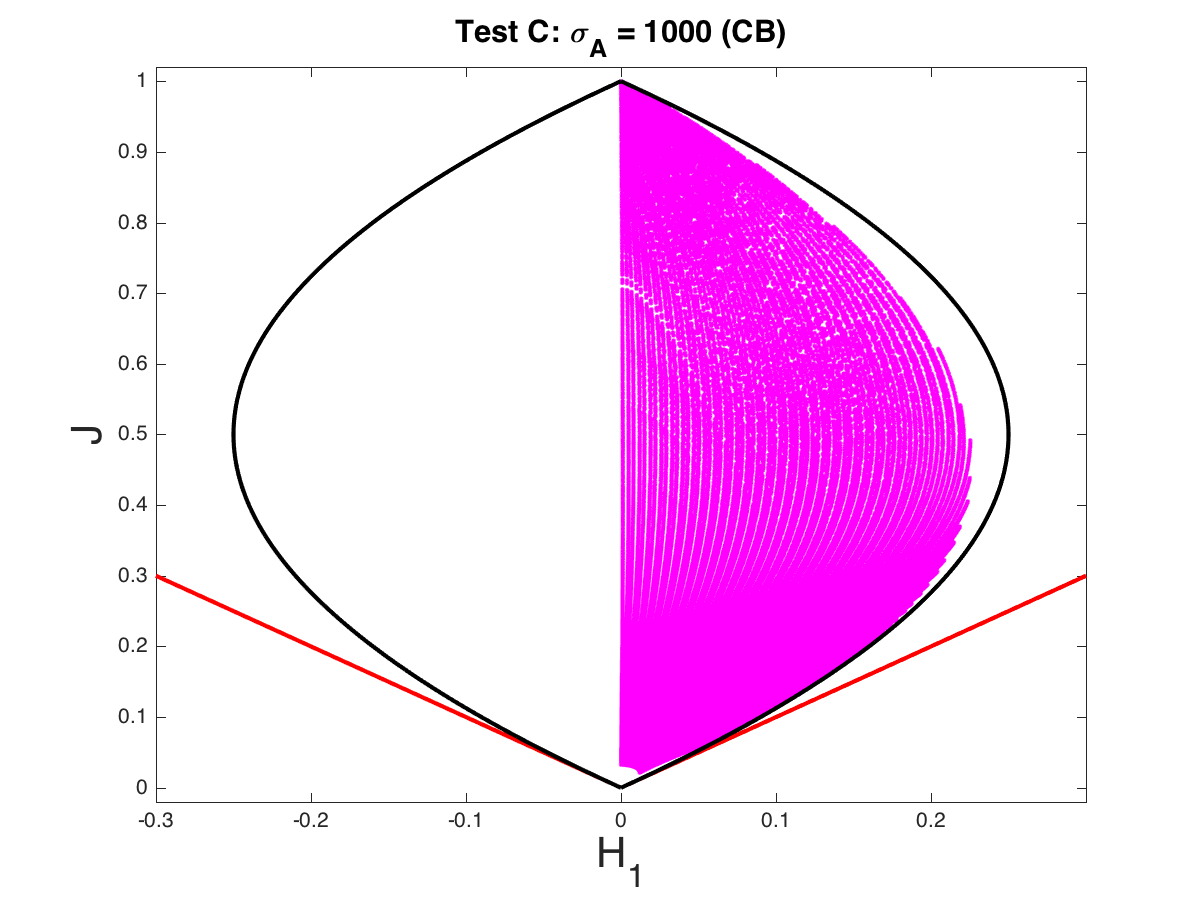
\includegraphics[width=0.5\textwidth]{figures/HomogeneousSphere_Realizability_Chi_1e3_CB}
    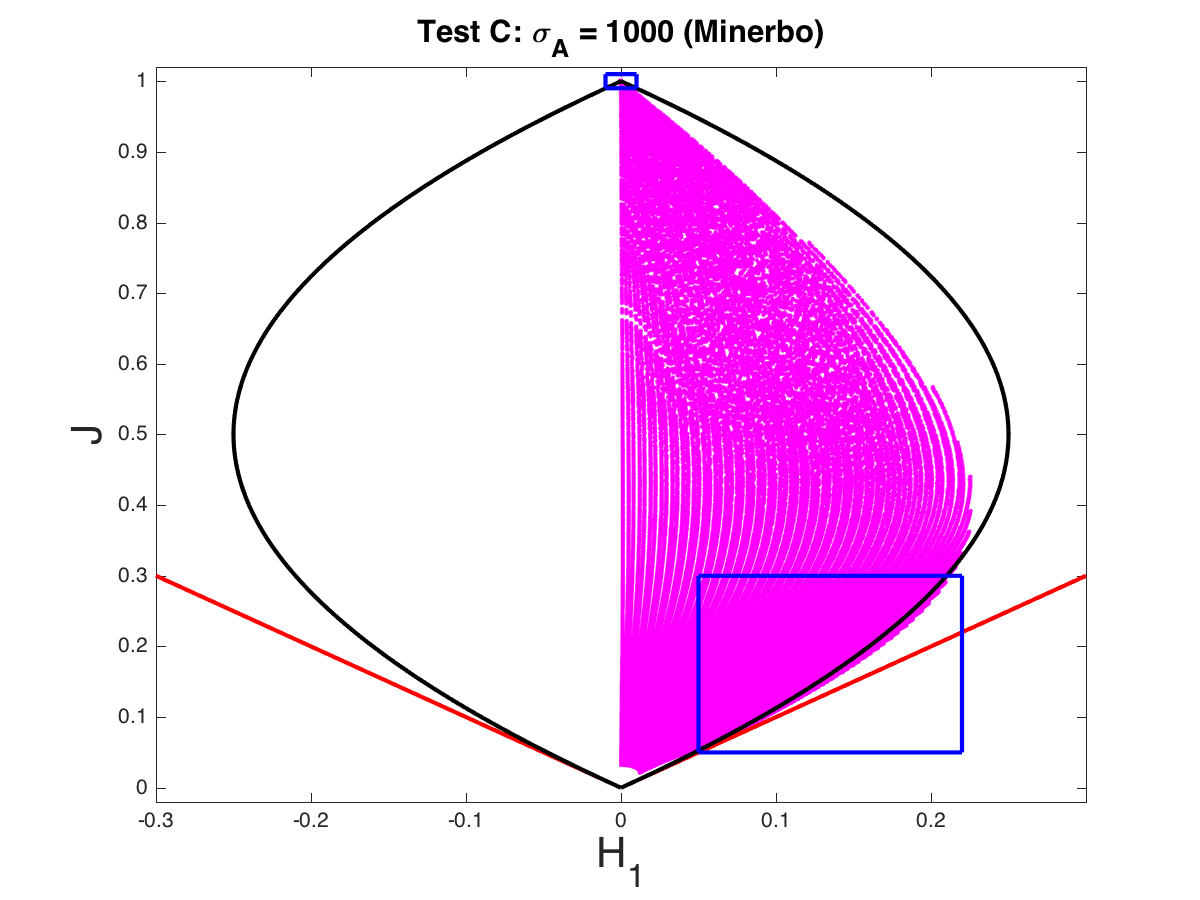
\includegraphics[width=0.5\textwidth]{figures/HomogeneousSphere_Realizability_Chi_1e3_Minerbo} \\
    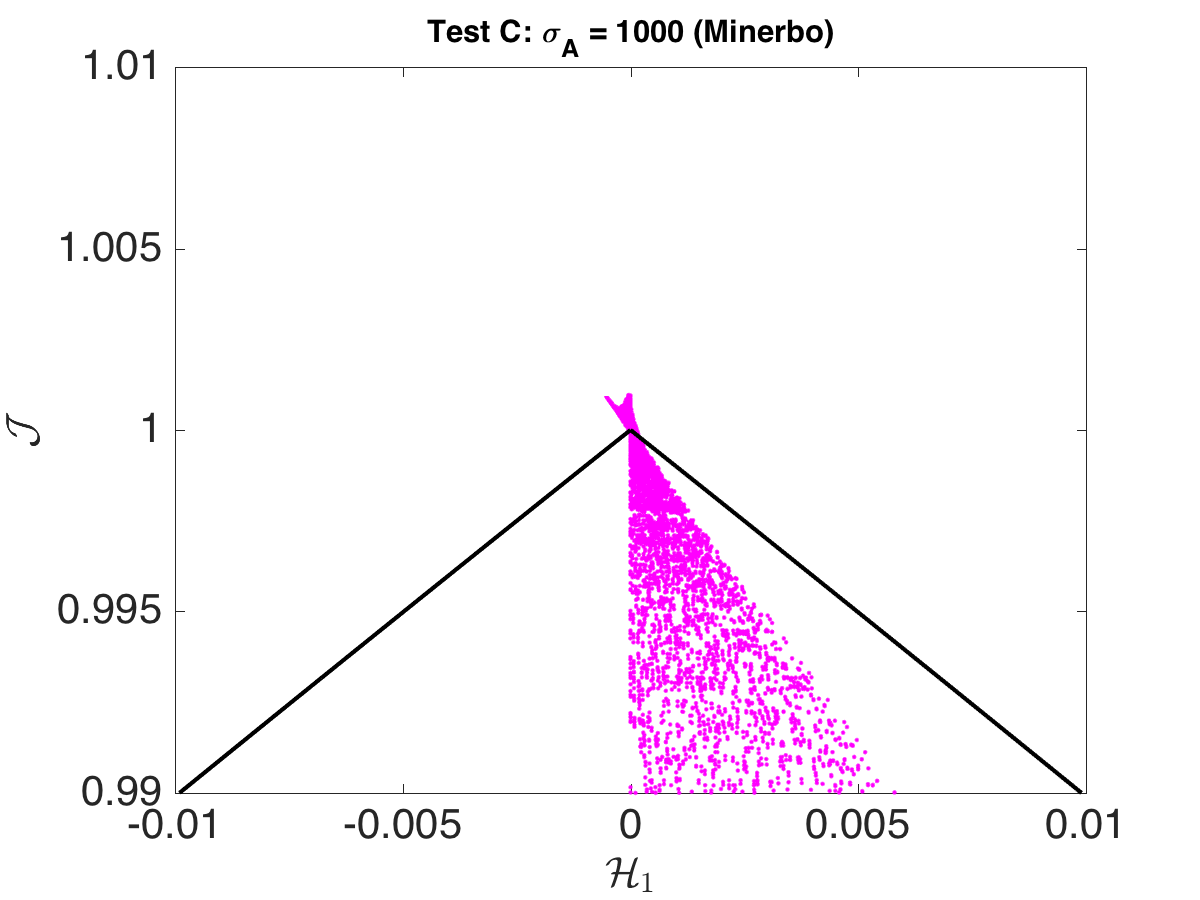
\includegraphics[width=0.5\textwidth]{figures/HomogeneousSphere_Realizability_Chi_1e3_Minerbo_Box1}
    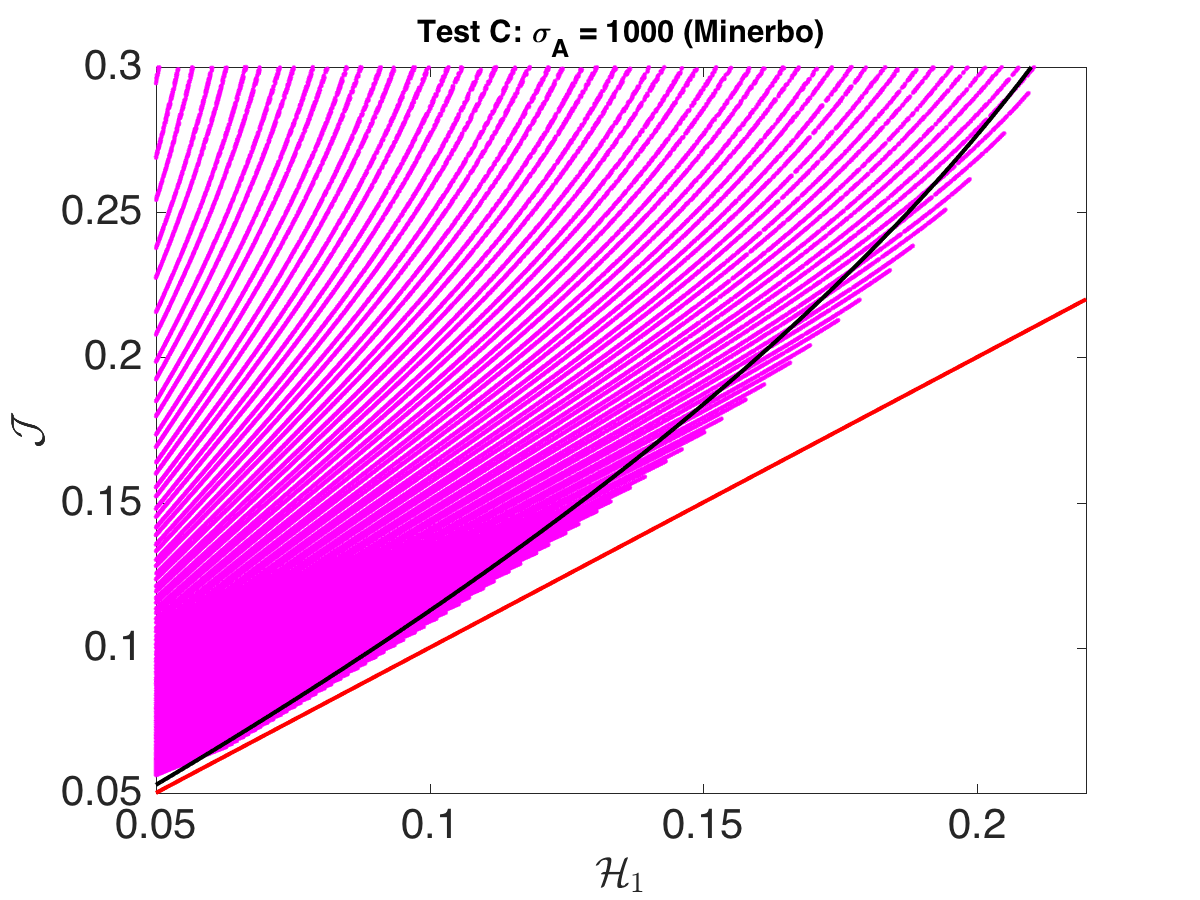
\includegraphics[width=0.5\textwidth]{figures/HomogeneousSphere_Realizability_Chi_1e3_Minerbo_Box2}
  \end{tabular}
   \caption{Plots of the numerical solution to the homogeneous sphere problem for Test~C in the $(\cH_{1},\cJ)$-plane.  Results obtained with the CB and Minerbo closures are plotted in the upper left and upper right panels, respectively.  Zoom-ins on the solutions obtained with the Minerbo closure are plotted in the lower two panels (cf. blue boxes in the upper right panel).  The boundaries of the realizable domains $\cR$ and $\cR^{+}$ are indicated with solid black and solid red curves, respectively.  See text for further details.  }
  \label{fig:HomogeneousSphereRealizability}
\end{figure}
As can be seen in the upper panels in Figure~\ref{fig:HomogeneousSphereRealizability}, the solution to the homogeneous sphere problem covers a large fraction of the right half of the realizable domain $\cR$, whose boundary is indicated by solid black curves in each panel.  
(The moments only appear in the right half of $\cR$ because we only compute in one octant.)  
When using the CB closure, the realizability-preserving DG-IMEX scheme developed here maintains solutions within $\cR$.  
When using the Minerbo closure, the appropriate realizable domain is given by $\cR^{+}$ (cf. Eq.~\eqref{eq:realizableSetPositive}), whose boundary is indicated by solid red lines in Figure~\ref{fig:HomogeneousSphereRealizability}, and we find that the numerical solution ventures outside $\cR$.  
Near the surface around $r=1$, the number density slightly exceeds unity (lower left panel), while for larger radii, the computed flux may exceed the value allowed by Fermi-Dirac statistics (lower right panel).  